\documentclass{article} % Defines the document class, article is commonly used
\usepackage[shortlabels]{enumitem}
\usepackage{amsmath}    % Allows for more advanced math formatting
\usepackage{amssymb}    % Provides additional mathematical symbols
\usepackage{amsthm}     % \qed
\usepackage{graphicx}   % image
\usepackage{float}      % image placement
\usepackage{hyperref}
\hypersetup{
    colorlinks=true,       % false: boxed links; true: colored links
    linkcolor=black,       % color of internal links
}
\usepackage[margin=1.5in]{geometry}

\begin{document}

\title{EEC133 Lab 1 Report}
\author{Tao Wang}
\date{\today}

\maketitle
\tableofcontents

\section*{Part 1}
\addcontentsline{toc}{section}{Part 1}
\begin{figure}[H]
    \centering
    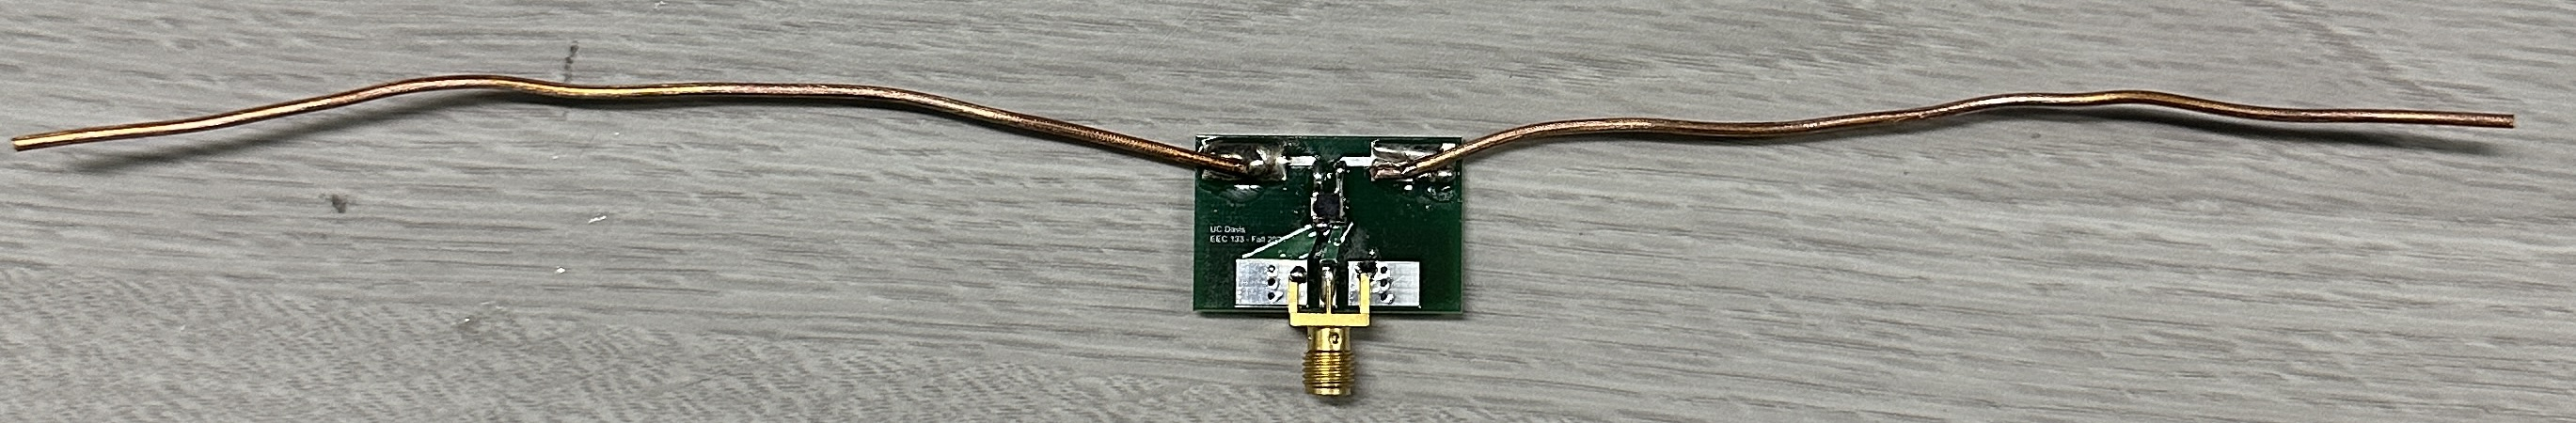
\includegraphics[width=1\textwidth]{./image/figure1.jpeg}
    \caption{Dipole Antenna}
\end{figure}

\section*{Part 2}
\addcontentsline{toc}{section}{Part 2}

\subsection*{Step 1}
\addcontentsline{toc}{subsection}{Step 1}
% \begin{figure}[H]
%     \centering
%     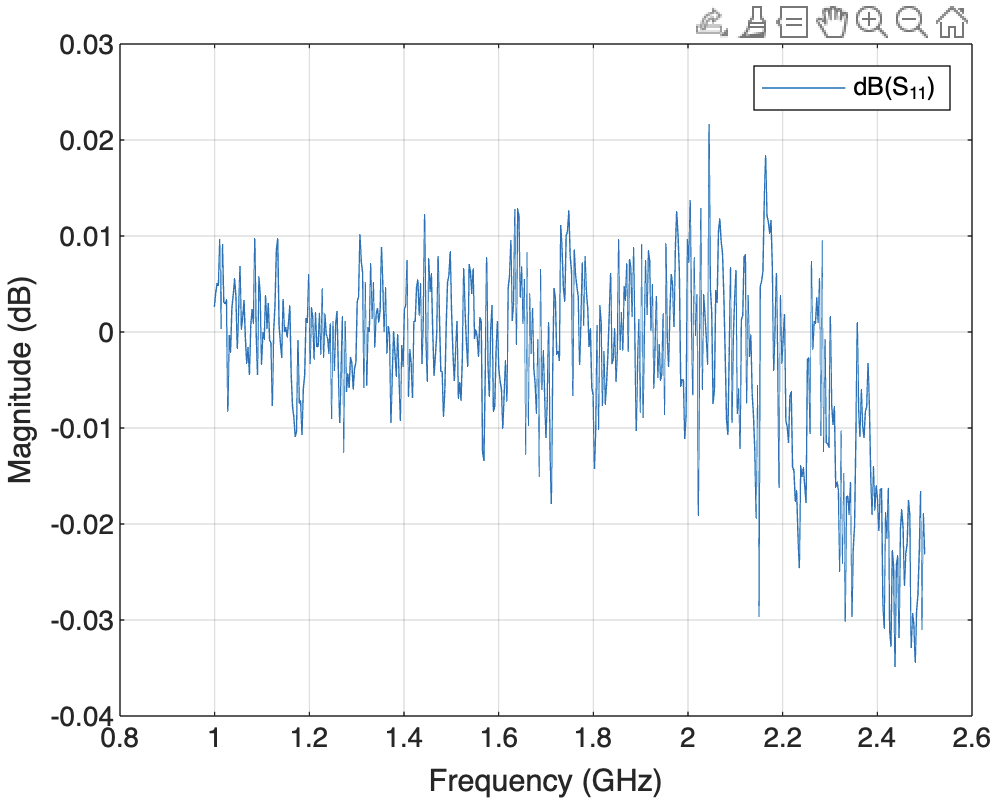
\includegraphics[width=1\textwidth]{./image/figure2.png}
%     \caption{$S_{11}$ of Unterminated Cable}
% \end{figure}

% \begin{figure}[H]
%     \centering
%     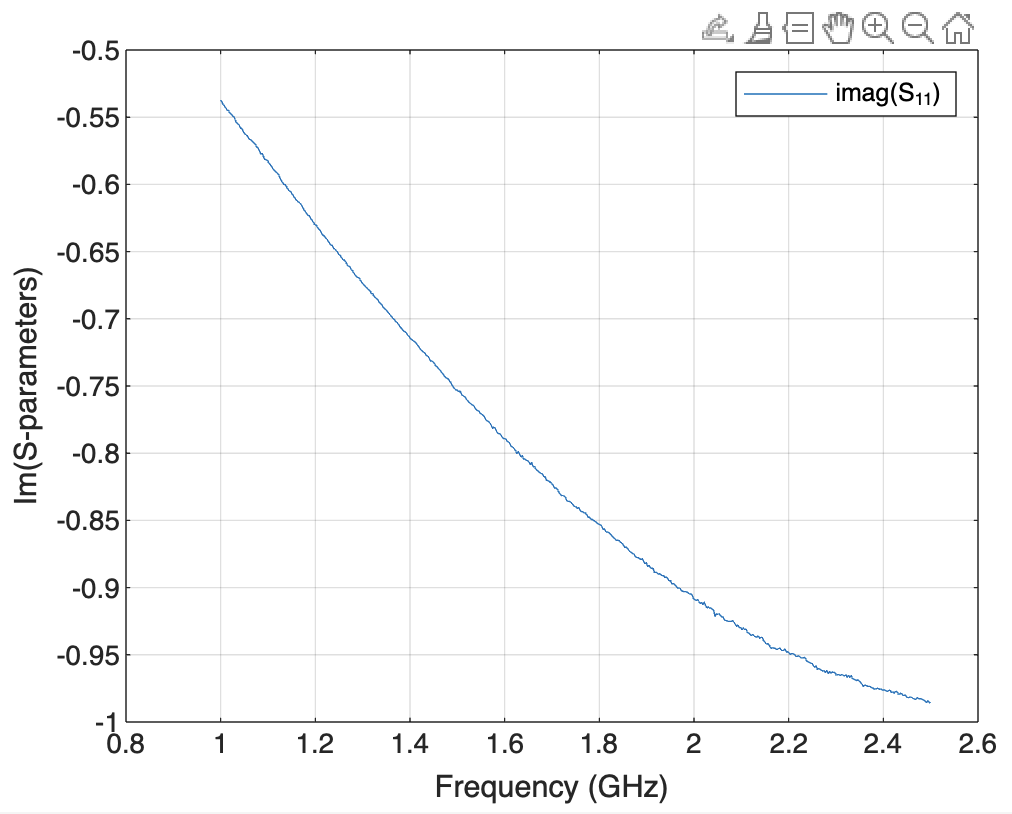
\includegraphics[width=1\textwidth]{./image/figure3.png}
%     \caption{Imaginary $S_{11}$ of Unterminated Cable}
% \end{figure}

\subsection*{Step 2}
\addcontentsline{toc}{subsection}{Step 2}

Cable Length: 25 inches long

\subsubsection*{Short Circuit S-Parameter}
\addcontentsline{toc}{subsubsection}{Short Circuit S-Parameter}
\begin{figure}[H]
    \centering
    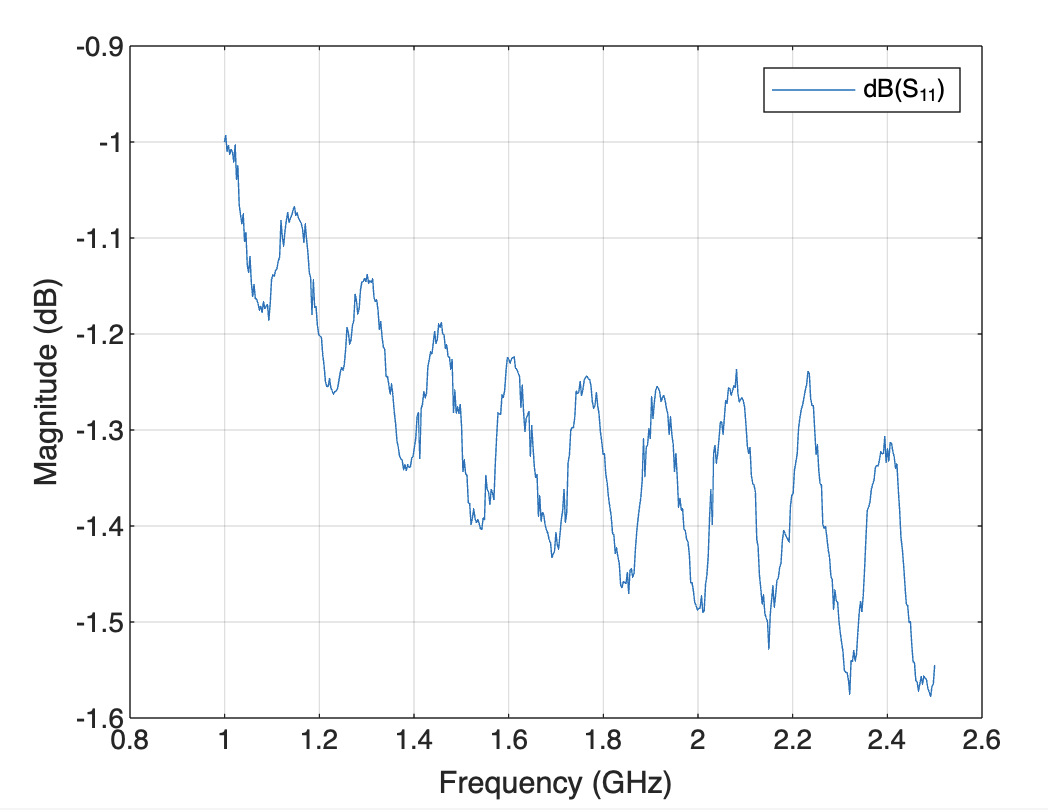
\includegraphics[width=0.5\textwidth]{./image/figure4.png}
    \caption{$S_{11}$ in a Short Circuit Transmission Line}
\end{figure}
\begin{figure}[H]
    \centering
    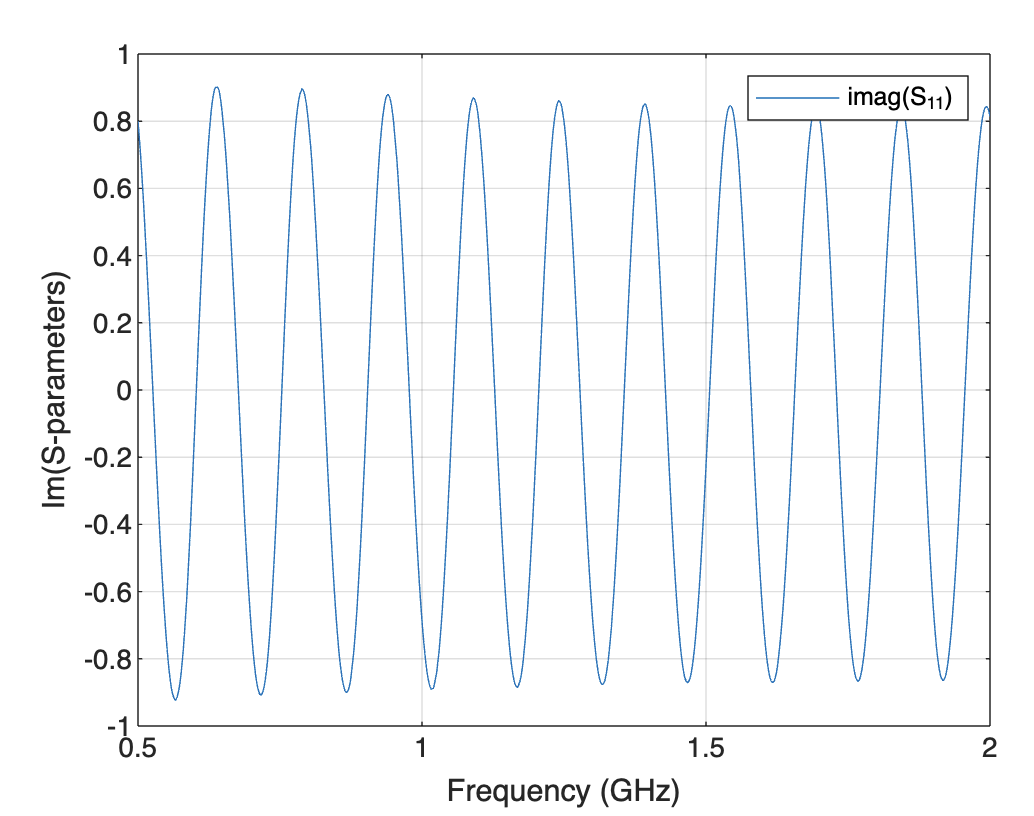
\includegraphics[width=0.5\textwidth]{./image/figure5.png}
    \caption{Reactance of $S_{11}$ in a Short Circuit Transmission Line}
\end{figure}

\subsubsection*{Open Circuit S-Parameter}
\addcontentsline{toc}{subsubsection}{Open Circuit S-Parameter}
\begin{figure}[H]
    \centering
    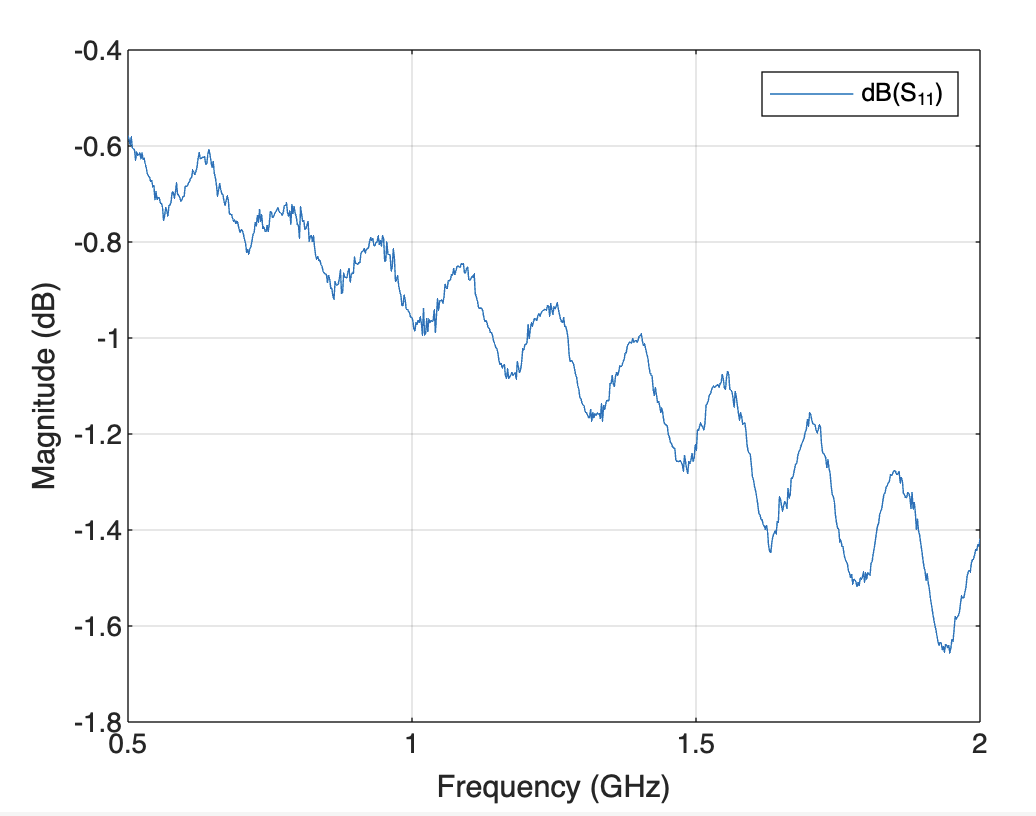
\includegraphics[width=0.5\textwidth]{./image/figure6.png}
    \caption{$S_{11}$ in a Open Circuit Transmission Line}
\end{figure}
\begin{figure}[H]
    \centering
    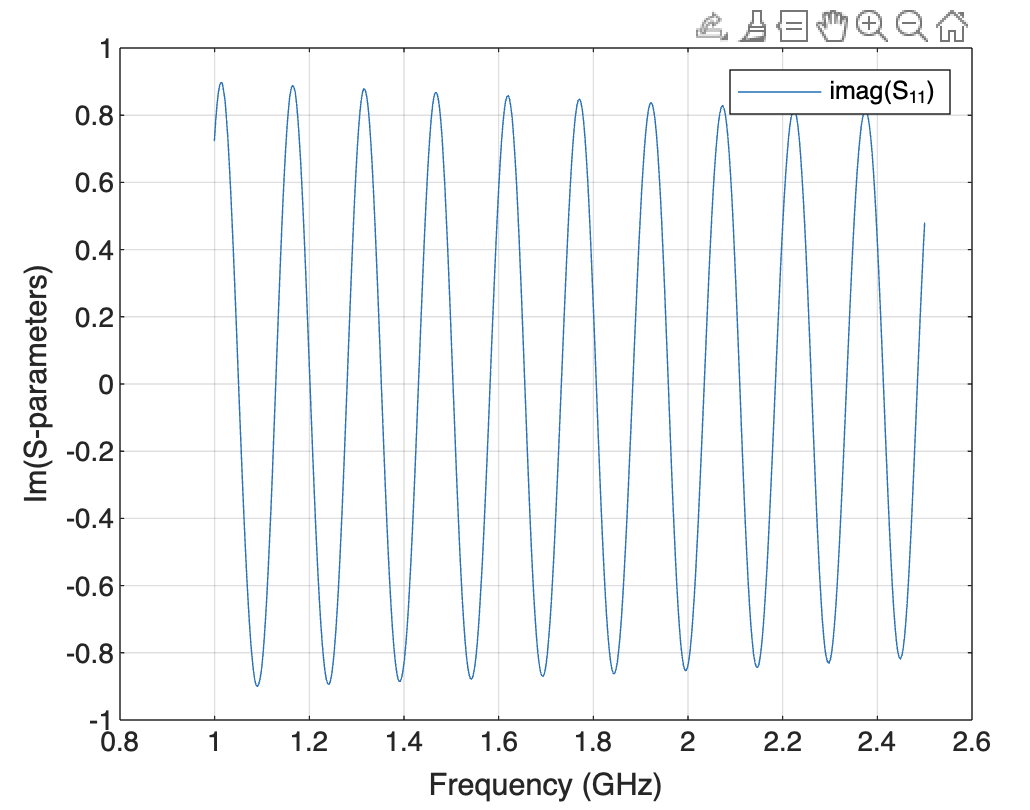
\includegraphics[width=0.5\textwidth]{./image/figure7.png}
    \caption{Reactance of $S_{11}$ in a Open Circuit Transmission Line}
\end{figure}

\subsubsection*{$50 \Omega$ Load Transmission Line S-Parameter}
\addcontentsline{toc}{subsubsection}{$50 \Omega$ Load Circuit S-Parameter}
\begin{figure}[H]
    \centering
    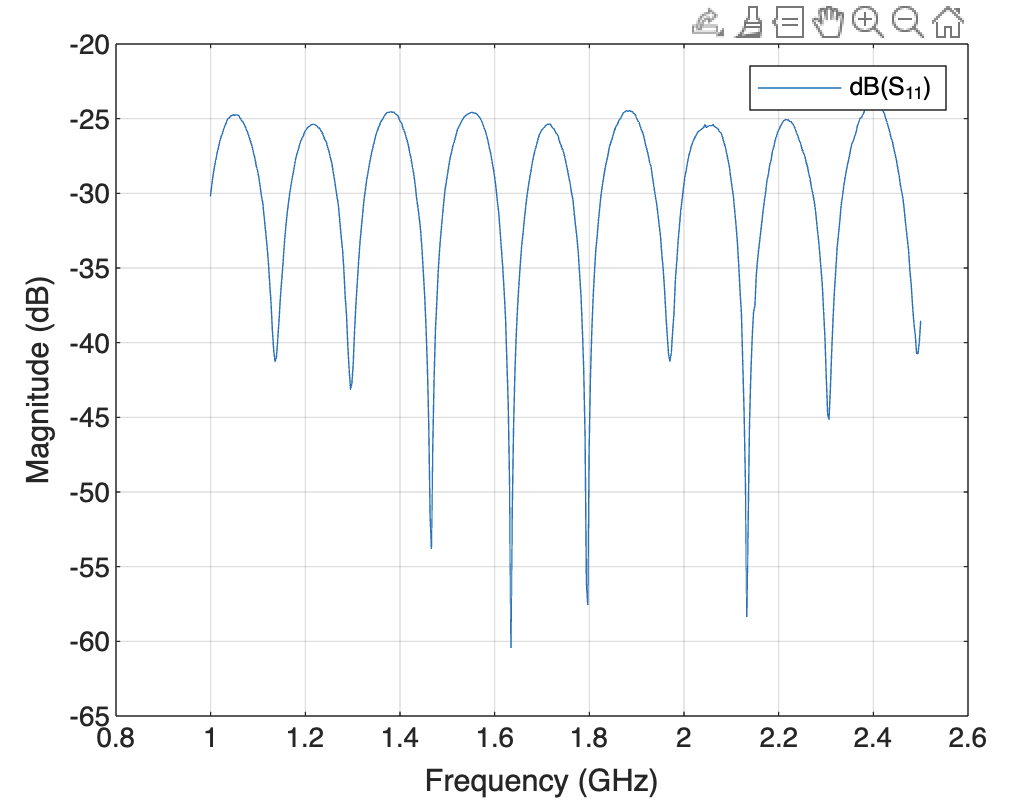
\includegraphics[width=0.5\textwidth]{./image/figure8.png}
    \caption{$S_{11}$ in a $50 \Omega$ Load Transmission Line}
\end{figure}
\begin{figure}[H]
    \centering
    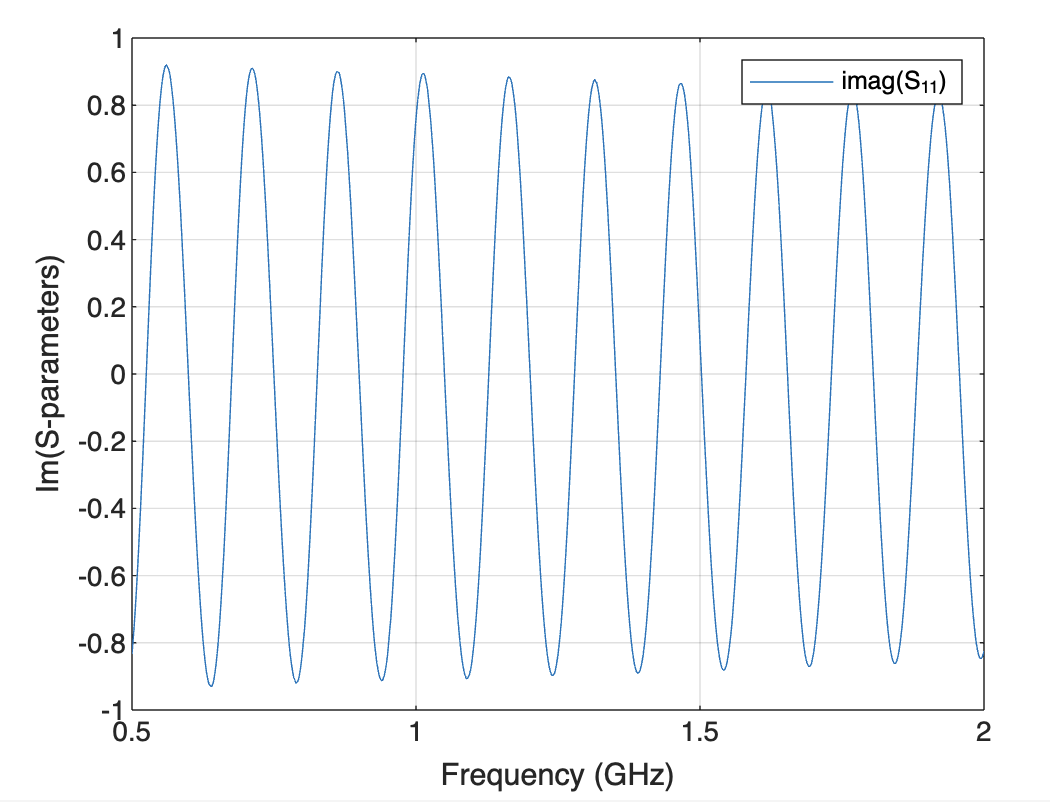
\includegraphics[width=0.5\textwidth]{./image/figure9.png}
    \caption{Reactance of $S_{11}$ in a $50 \Omega$ Load Circuit Transmission Line}
\end{figure}

\section*{Part 3}
\addcontentsline{toc}{section}{Part 3}
\subsection*{Step 1}
\addcontentsline{toc}{subsection}{Step 1}
\begin{figure}[H]
    \centering
    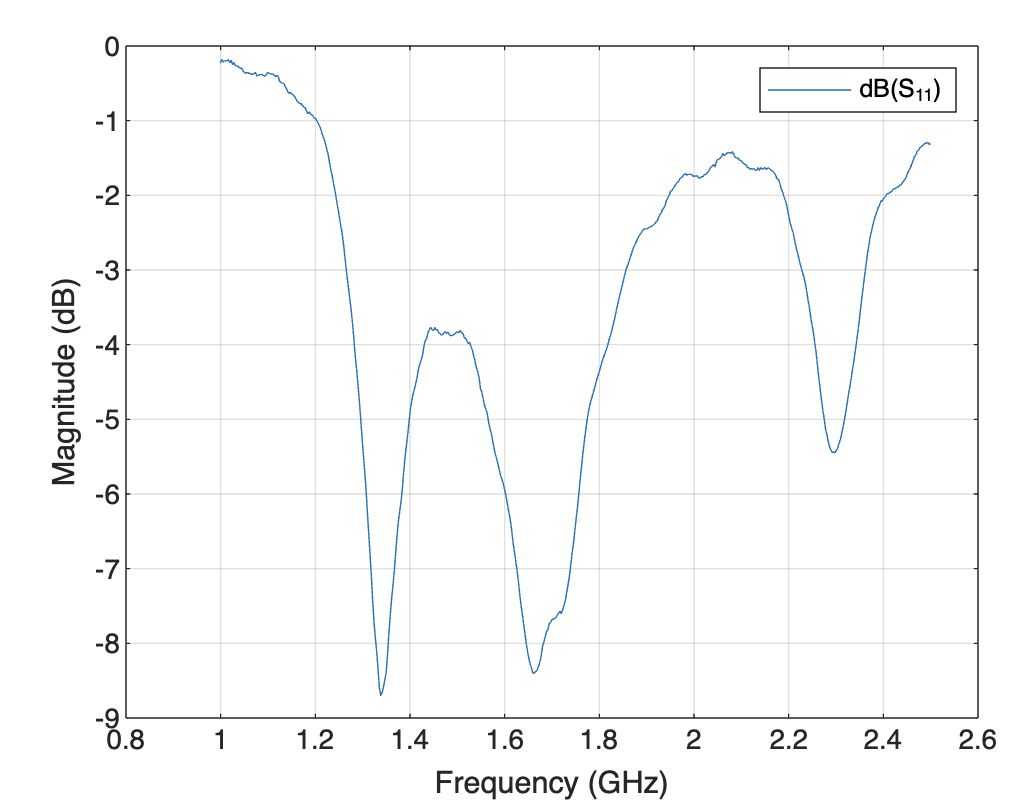
\includegraphics[width=0.5\textwidth]{./image/figure10.png}
    \caption{Dipole Antenna's $S_{11}$ Magnitude}
\end{figure}
\begin{figure}[H]
    \centering
    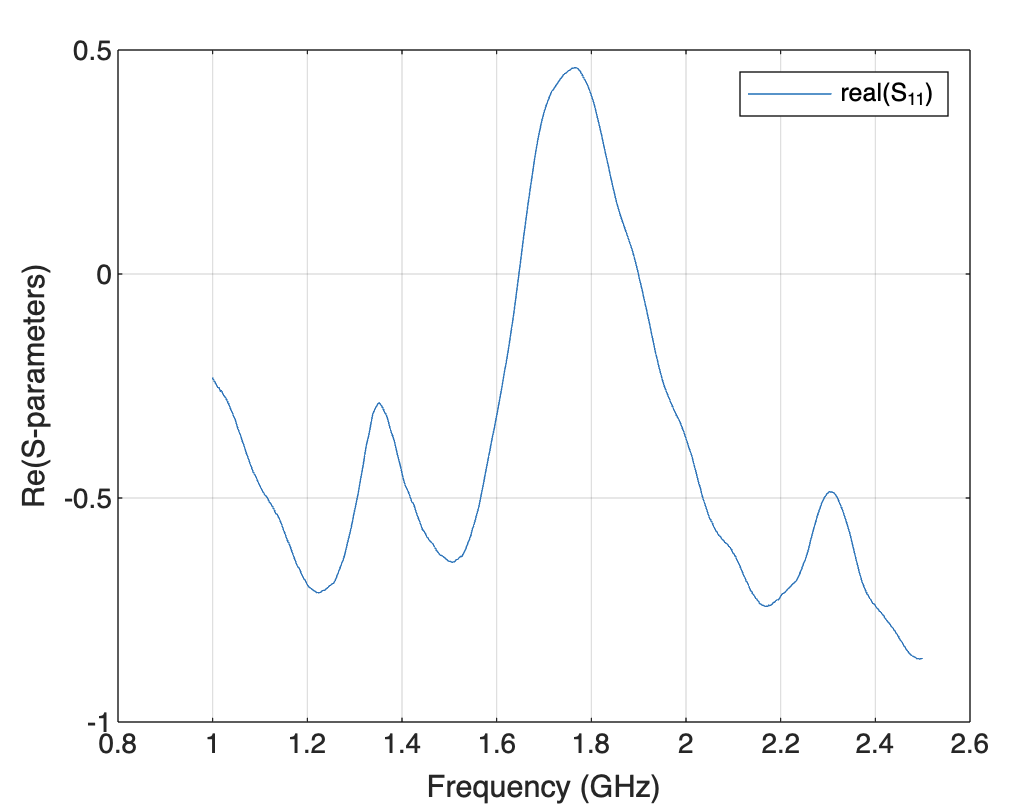
\includegraphics[width=0.5\textwidth]{./image/figure11.png}
    \caption{Dipole Antenna's Real Part of $S_{11}$}
\end{figure}
\begin{figure}[H]
    \centering
    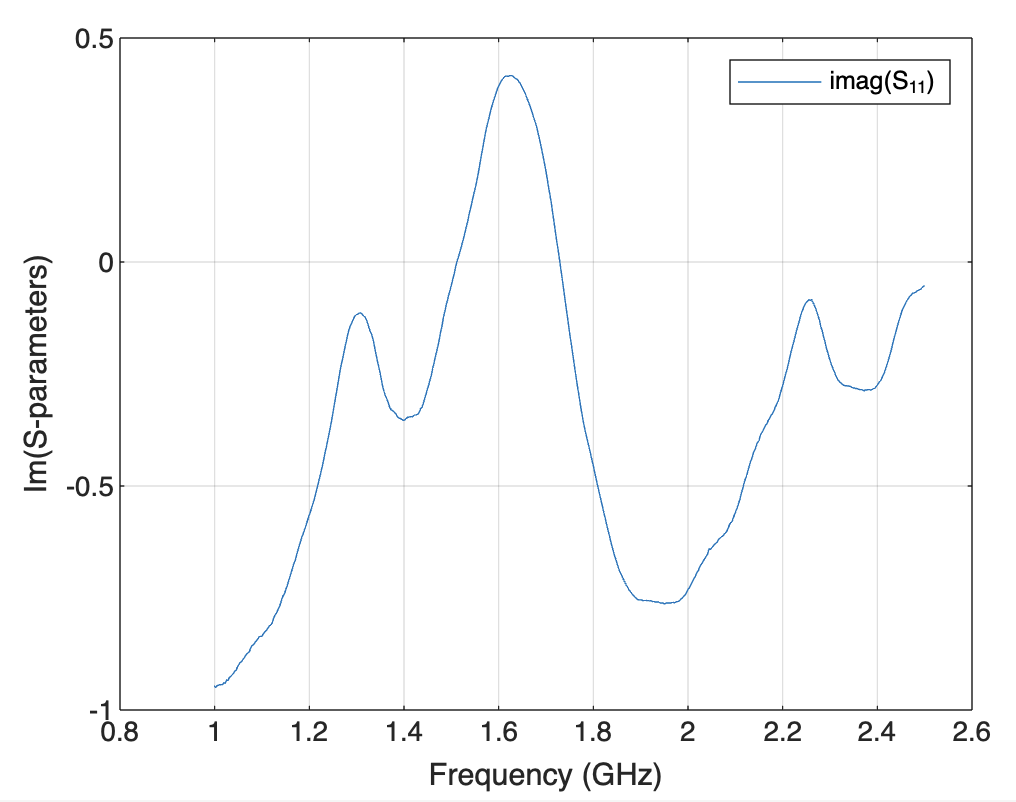
\includegraphics[width=0.5\textwidth]{./image/figure12.png}
    \caption{Dipole Antenna's Imaginary Part of $S_{11}$}
\end{figure}

\subsection*{Step 2}
\addcontentsline{toc}{subsection}{Step 2}
Distance between the two antennas: 10 feet.

\subsection*{Step 3}
\addcontentsline{toc}{subsection}{Step 3}

\begin{table}[h!]
    \centering
    \begin{tabular}{|c|c|}
        \hline
        \textbf{Angle (degrees)} & \textbf{$S_{21}$ (dB)} \\
        \hline
        0                        & -48.0                  \\
        10                       & -53.0                  \\
        20                       & -50.0                  \\
        30                       & -54.8                  \\
        40                       & -53.0                  \\
        50                       & -45.0                  \\
        60                       & -45.04                 \\
        70                       & -48.0                  \\
        80                       & -54.0                  \\
        90                       & -64.0                  \\
        100                      & -55.0                  \\
        110                      & -47.0                  \\
        120                      & -44.0                  \\
        130                      & -44.0                  \\
        140                      & -44.6                  \\
        150                      & -45.6                  \\
        160                      & -48.0                  \\
        170                      & -50.0                  \\
        180                      & -56.0                  \\
        \hline
    \end{tabular}
    \caption{$S_{21}$ values at different angles}
\end{table}

\subsection*{Step 4}
\addcontentsline{toc}{subsection}{Step 4}
$S_{21} = -64 dB$

\section*{Part 4}
\addcontentsline{toc}{section}{Part 4}
\subsection*{1}
\addcontentsline{toc}{subsection}{1}

\subsection*{2}
\addcontentsline{toc}{subsection}{2}

\subsection*{3}
\addcontentsline{toc}{subsection}{3}

\subsection*{5}
\addcontentsline{toc}{subsection}{5}

\end{document}
